\documentclass{article}
\usepackage{tikz}
\usetikzlibrary{arrows.meta, positioning, fit, calc}

\begin{document}

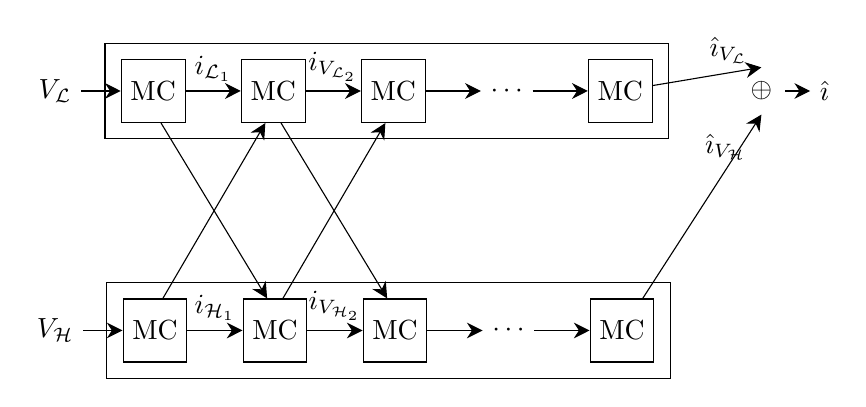
\begin{tikzpicture}[
    box/.style={draw, minimum width=0.8cm, minimum height=0.8cm},
    arrow/.style={-{Stealth[length=2mm, width=2mm]}},
    node distance=0.7cm
]

% Top row (low resolution)
\node[left] (VL) {$\text{V}_\mathcal{L}$};
\node[box, right=0.5cm of VL] (MC1L) {MC};
\node[box, right=of MC1L] (MC2L) {MC};
\node[box, right=of MC2L] (MC3L) {MC};
\node[right=of MC3L] (dotsL) {$\cdots$};
\node[box, right=of dotsL] (MC4L) {MC};

% Bottom row (high resolution)
\node[left, below=2.5cm of VL] (VH) {$\text{V}_\mathcal{H}$};
\node[box, right=0.5cm of VH] (MC1H) {MC};
\node[box, right=of MC1H] (MC2H) {MC};
\node[box, right=of MC2H] (MC3H) {MC};
\node[right=of MC3H] (dotsH) {$\cdots$};
\node[box, right=of dotsH] (MC4H) {MC};

% Final output
\node[right=2cm of MC4L] (output) {$\hat{\imath}$};

% Draw rectangles around the rows
\node[draw, fit=(MC1L) (MC4L), inner sep=0.2cm] (topRect) {};
\node[draw, fit=(MC1H) (MC4H), inner sep=0.2cm] (bottomRect) {};

% Horizontal arrows for top row
\draw[arrow] (VL) -- (MC1L);
\draw[arrow] (MC1L) -- node[above] {$i_{\mathcal{L}_1}$} (MC2L);
\draw[arrow] (MC2L) -- node[above] {$i_{\text{V}_{\mathcal{L}_2}}$} (MC3L);
\draw[arrow] (MC3L) -- (dotsL);
\draw[arrow] (dotsL) -- (MC4L);

% Horizontal arrows for bottom row
\draw[arrow] (VH) -- (MC1H);
\draw[arrow] (MC1H) -- node[above] {$i_{\mathcal{H}_1}$} (MC2H);
\draw[arrow] (MC2H) -- node[above] {$i_{\text{V}_{\mathcal{H}_2}}$} (MC3H);
\draw[arrow] (MC3H) -- (dotsH);
\draw[arrow] (dotsH) -- (MC4H);

% Diagonal arrows for cross-connections
\draw[arrow] ($(MC1L.south)+(0.1,0)$) -- ($(MC2H.north)-(0.1,0)$);
\draw[arrow] ($(MC1H.north)+(0.1,0)$) -- ($(MC2L.south)-(0.1,0)$);
\draw[arrow] ($(MC2L.south)+(0.1,0)$) -- ($(MC3H.north)-(0.1,0)$);
\draw[arrow] ($(MC2H.north)+(0.1,0)$) -- ($(MC3L.south)-(0.1,0)$);

% Final output arrows
\draw[arrow] (MC4L) -- node[above, pos=0.7] {$\hat{\imath}_{\text{V}_\mathcal{L}}$} ($(output) + (-0.8, 0.3)$);
\draw[arrow] (MC4H) -- node[above, pos=0.7] {$\hat{\imath}_{\text{V}_\mathcal{H}}$} ($(output) + (-0.8, -0.3)$);

% Add the plus symbol
\node at ($(output) + (-0.8, 0)$) {$\oplus$};

% Final arrow
\draw[arrow] ($(output) + (-0.5, 0)$) -- (output);

\end{tikzpicture}

\end{document}